\chapter{Rešerše}
\label{0-reserse}

Tarifní pásma Pražské integrované dopravy jsou mimo jiné publikována jako shapefile 
\footnote{formát vektorového datového úložiště Esri pro ukládání umístění,
tvaru a atributů geografických prvků \cite{shapefile}}
na portálu \textit{opendata hlavního města Prahy} \cite{opendata}. Tento shapefile
obsahuje vektorové vrstvy polygonů.

První myšlenkou, jak se přiblížit k takovým polygonům bylo vytvoření linií mezi jednotlivými zastávkami.
K tomu slouží takzvaná triangulace, která vytvoří trojúhelníky bezi body, kde uvnitř těchto trojuhelníků  
už neleží žádné body a každý trojúhelník má vždy společnou jednu hranu. 

Takové triangulace se používají v kartografii, tak v GIS, v Dálkovém průzkumu země,
počítačové grafice, při analýze vlastností a struktury materiálů, plánování pohybu robotů
nebo při modelování přírodních jevů. \cite{bayer-delaunay}

Existuje více druhů triangulací, které využívají vždy jinou metodu konstrukce
a mají rozdílný výpočetní stupeň složitosti. 

Hladová (Greedy) triangulace se snaží vytvářet trojúhelníky s nejkratšími stranami,
které nesplňují žádnou speciální geometrickou podmínku. Její realizace je jednoduchá,
avšak důsledek toho jsou často tvarově nepěkné nebo nevhodné trojúhelníky. Má velkou výpočetní
složitost \(O(n^3)\), lze optimalizovat na \(O(n^2 \log(n))\) a v kartografii se 
nepříliš používá. \cite{vanicek}

\begin{figure}[H] \centering
    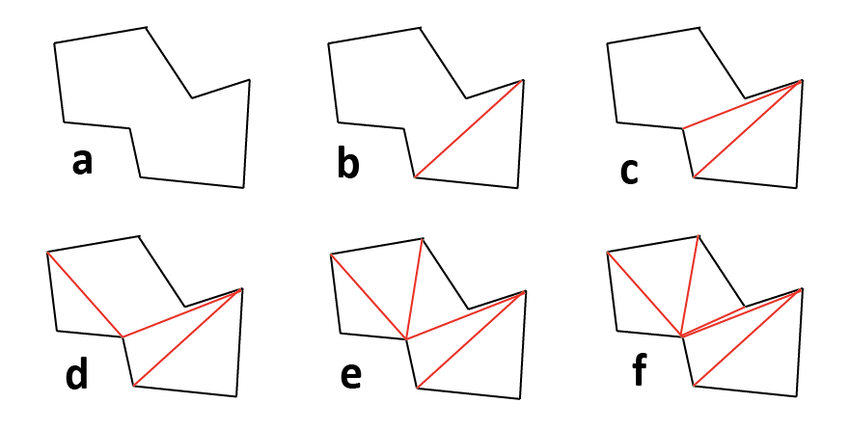
\includegraphics[width=400pt]{./pictures/triangulace-greedy.png}
    \caption[Ilustrace Greedy triangulace]{Ilustrace Greedy triangulace \cite{triangulace-greedy}}
	\label{fig:triangulace-greedy}              
\end{figure}

Další triangulací je tzv. Delaunay triangulace, která je nejčastěji používaná triangulace.
Delaunay triangulace je vytváření liniových spojnic bodů mez jednotlivými body, které si jsou sobě nejblíž,
za pomocí opsaných kružnic. Delaunay triangulace má několik vlastností. Jednou z nich je například,
že uvnitř kružnice k opsané libovolnému trojúhelníku neleží žádný jiný bod.
Zároveň Delaunay triangulace je jednoznačná, pokud žádné čtyři body neleží na kružnici.
Na rozdíl od Greedy triangulace nehodnotí kritérium délky hran. Díky maximalizaci minimálních
úhlů vytváří takové trojúhelníky, které se nejvíc blíží k rovnostranným trojúhelníkům, 
což znamená, že se snaží eliminovat trojúhelníky, které jsou ostroúhlé.

Pro výtváření konstrukce Delaunay triangulace jsou k dispozici různé algoritmy: lokální prohazování, 
inkrementální konstrukce, inkrementální vkládání, rozděl a panuj nebo sweep line. \cite{bayer-delaunay}

\begin{figure}[H] \centering
    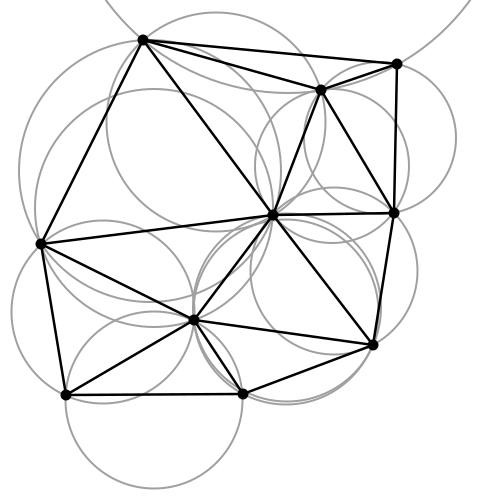
\includegraphics[width=280pt]{./pictures/triangulace-delaunay.png}
    \caption[Ilustrace Delaunay triangulace]{Ilustrace Delaunay triangulace \cite{triangulace-delaunay}}
	\label{fig:triangulace-delaunay}              
\end{figure}



Další nápadem byla aplikace Voronoi diagram algoritmu, což je způsob dekompozice 
metrického prostoru určený vzdálenostmi k dané diskrétní množině bodů v prostoru.
Tento algoritmus má taky několik vlastností, jež budou prezentovány v dalších kapitolách 
(viz \ref{voronoi-vlastnosti}). 